\documentclass[12pt,a4paper]{report}

% Bahasa & font (XeTeX)
\usepackage{fontspec}
\setmainfont{Times New Roman}
\setsansfont{Arial}
\setmonofont{Consolas}
\usepackage[indonesian]{babel}
\addto\captionsindonesian{\renewcommand{\bibname}{Daftar Pustaka}}

% Tata letak halaman
\usepackage[top=3cm,bottom=3cm,left=3.5cm,right=2.5cm]{geometry}
\setlength{\headheight}{15pt}
\usepackage{setspace}
\onehalfspacing
\usepackage{parskip}
\usepackage{fancyhdr}
\usepackage{titlesec}

% Tabel, matematika, dan grafis
\usepackage{amsmath,amssymb}
\usepackage{graphicx}
\usepackage{booktabs}
\usepackage{longtable}
\usepackage{array}
\usepackage{tabularx}
\usepackage{multirow}
\usepackage{float}
\usepackage{caption}
\usepackage{xcolor}
\usepackage{tikz}
\usetikzlibrary{arrows.meta,positioning,shapes.geometric,fit,backgrounds}

% Listing kode & kotak terminal
\usepackage{listings}
\usepackage[most]{tcolorbox}

% Hyperref (muat paling akhir)
\usepackage[hidelinks,unicode]{hyperref}

% Warna netral akademis
\definecolor{MutedGray}{HTML}{555555}
\definecolor{CodeBg}{HTML}{F8F8F8}
\definecolor{CodeBorder}{HTML}{CCCCCC}
\definecolor{CodeKw}{HTML}{000099}
\definecolor{CodeStr}{HTML}{A31515}

% Format judul bab
\titleformat{\chapter}[display]
  {\normalfont\bfseries}
  {\large\chaptertitlename\ \thechapter}
  {4pt}
  {\Large}
\titlespacing*{\chapter}{0pt}{-10pt}{18pt}

\titleformat{\section}
  {\normalfont\large\bfseries}
  {\thesection}{0.8em}{}
\titleformat{\subsection}
  {\normalfont\normalsize\bfseries}
  {\thesubsection}{0.8em}{}

% Header dan footer
\pagestyle{fancy}
\fancyhf{}
\fancyhead[L]{\small Tugas 2 --- Kecerdasan Artifisial}
\fancyhead[R]{\small Kelompok 5}
\fancyfoot[C]{\small\thepage}
\renewcommand{\headrulewidth}{0.4pt}
\fancypagestyle{plain}{
  \fancyhf{}
  \fancyfoot[C]{\small\thepage}
  \renewcommand{\headrulewidth}{0pt}
}

% Konfigurasi listings untuk Prolog
\lstdefinelanguage{PrologCustom}{
  morekeywords={is,not,true,fail,forall,findall,maplist,foldl,member,memberchk,
                once,catch,throw,setup_call_cleanup,retractall,assertz,asserta,
                use_module,encoding,thread_local,ensure_loaded,http_handler,
                http_server,http_reply_file,http_read_json_dict,reply_json_dict},
  sensitive=true,
  morecomment=[l]{\%},
  morestring=[b]",
  morestring=[b]'
}

\lstset{
  language=PrologCustom,
  basicstyle=\ttfamily\footnotesize,
  keywordstyle=\bfseries\color{CodeKw},
  commentstyle=\itshape\color{MutedGray},
  stringstyle=\color{CodeStr},
  numbers=left,
  numberstyle=\tiny\color{MutedGray},
  stepnumber=1,
  numbersep=8pt,
  backgroundcolor=\color{CodeBg},
  frame=single,
  rulecolor=\color{CodeBorder},
  breaklines=true,
  breakatwhitespace=false,
  tabsize=4,
  showstringspaces=false,
  captionpos=b,
  literate={—}{{\textemdash}}1 {–}{{\textendash}}1 {−}{{-}}1
}

% Kotak terminal untuk transkrip konsol
\newtcolorbox{consolebox}[1][]{
  colback=CodeBg,
  colframe=CodeBorder,
  colupper=black,
  coltitle=black,
  colbacktitle=gray!15,
  fonttitle=\bfseries\small,
  fontupper=\scriptsize,
  arc=2pt,
  boxrule=0.6pt,
  left=8pt,right=8pt,top=5pt,bottom=5pt,
  breakable,
  title=#1
}

\captionsetup{font=small,labelfont=bf}
\newcolumntype{Y}{>{\raggedright\arraybackslash}X}
\emergencystretch=2em

\begin{document}

% ============================================================================
% HALAMAN SAMPUL
% ============================================================================
\begin{titlepage}
\begin{center}
\vspace*{0.8cm}

{\fontsize{17}{22}\selectfont\bfseries SISTEM PAKAR DIAGNOSA DINI\\PENYAKIT TETELO (\textit{NEWCASTLE DISEASE})\\PADA AYAM BERBASIS PROLOG\par}
\vspace{0.45cm}
{\fontsize{14}{19}\selectfont\bfseries LAPORAN TUGAS 2\par}

\vspace{1.6cm}

{\fontsize{12}{16}\selectfont Disusun oleh:\par}
\vspace{0.2cm}
{\fontsize{13}{17}\selectfont\bfseries Kelompok 5\par}
\vspace{0.5cm}

{\fontsize{12}{15}\selectfont
\textbf{ARDIAN}\\
NPM. 260820701100008\\[0.3cm]
\textbf{MUHAMMAD ICHSAN}\\
NPM. 260820701100007\\[0.3cm]
\textbf{IRFAN SYAHPUTRA}\\
NPM. 2308107010030\par}

\vfill


\includegraphics[width=3.8cm]{images/unsyiah.png}

\vfill

{\fontsize{12}{16}\selectfont\bfseries
PROGRAM STUDI KECERDASAN BUATAN DEPARTEMEN INFORMATIKA\\
FAKULTAS MATEMATIKA DAN ILMU PENGETAHUAN ALAM\\
UNIVERSITAS SYIAH KUALA\\
2026\par}

\end{center}
\end{titlepage}

% ============================================================================
% DAFTAR ISI, TABEL, GAMBAR
% ============================================================================
\pagenumbering{roman}
\tableofcontents
\clearpage
\listoftables
\listoffigures
\clearpage

\pagenumbering{arabic}

% ============================================================================
% BAB I: PENDAHULUAN
% ============================================================================
\chapter{Pendahuluan}

\section{Latar Belakang Masalah}
Sektor peternakan ayam merupakan salah satu komoditas utama penyedia protein hewani di Indonesia, baik dalam bentuk daging maupun telur. Meskipun pertumbuhan populasi ternak ayam terus meningkat, usaha peternakan menghadapi risiko kerugian ekonomi yang tinggi akibat serangan penyakit infeksius unggas, salah satunya adalah penyakit \textbf{Tetelo} atau \textit{Newcastle Disease} (ND)~\cite{azzahra2026,ahsyar2021}. Sebagai gambaran, data kematian unggas di Kabupaten Purwakarta yang dilaporkan oleh Azzahra dkk.~\cite{azzahra2026} mencatat 78 kasus kematian akibat Tetelo pada tahun 2022, 21 kasus pada tahun 2023, dan 13 kasus pada tahun 2024.

Tingginya dampak penyakit unggas di tingkat peternak dipicu oleh dua kendala utama: keterbatasan pengetahuan peternak dalam mengenali gejala klinis secara dini serta terbatasnya akses terhadap dokter hewan, terutama dari sisi biaya, waktu tempuh, dan ketersediaan tenaga medis hewan di daerah pedesaan~\cite{ahsyar2021}. Keterlambatan identifikasi gejala awal berisiko memperluas penularan penyakit dalam satu kandang sebelum penanganan lapangan dilakukan.

Salah satu pendekatan kecerdasan artifisial yang relevan untuk membantu skrining awal adalah \textbf{sistem pakar berbasis aturan (\textit{rule-based expert system})}. Dengan merepresentasikan pengetahuan mengenai gejala klinis dan aturan diagnosis ke dalam bahasa pemrograman logika seperti \textbf{Prolog}, sistem dapat melakukan penelusuran penalaran secara terstruktur dan konsisten. Penggabungan mesin inferensi \textit{Backward Chaining} dengan metode \textit{Certainty Factor} (CF) memungkinkan sistem tidak hanya mencocokkan kombinasi gejala yang teramati, tetapi juga mengkuantifikasi tingkat dukungan bukti terhadap pola gejala yang muncul.

\section{Tujuan Proyek}
Tujuan utama proyek ini adalah:
\begin{enumerate}
  \item Merancang dan membangun basis pengetahuan sistem pakar untuk skrining dini penyakit Tetelo pada ayam yang terdiri atas 12 gejala klinis, 4 kategori keluaran, dan 15 aturan \texttt{IF--THEN}.
  \item Mengimplementasikan mesin inferensi \textbf{Backward Chaining} yang terintegrasi dengan perhitungan \textbf{Certainty Factor (CF)} menggunakan bahasa pemrograman SWI-Prolog pada berkas \texttt{diagnosa\_tetelo.pl}.
  \item Menyediakan antarmuka konsol interaktif Prolog sebagai antarmuka utama serta antarmuka web lokal (\texttt{web/server.pl}) yang berbagi basis pengetahuan dan mesin inferensi yang sama untuk memudahkan penggunaan dan transparansi perhitungan aturan.
  \item Menguji fungsionalitas sistem, ketepatan perhitungan CF, mekanisme \textit{tie-breaker}, serta penanganan input menggunakan skenario uji \textit{black-box} dan \textit{walkthrough}.
\end{enumerate}

\section{Batasan Proyek}
Agar ruang lingkup pengerjaan tetap terarah, ditetapkan beberapa batasan berikut:
\begin{enumerate}
  \item Sistem difokuskan khusus untuk \textbf{skrining dini penyakit Tetelo (\textit{Newcastle Disease}) pada ayam} dan tidak mencakup diagnosis banding penyakit unggas lain (seperti Flu Burung, Snot, atau Gumboro).
  \item Kategori keluaran \texttt{D1}--\texttt{D3} merepresentasikan \textbf{pola aturan proyek} (umum; pernapasan/pencernaan/produksi; saraf/gangguan gerak), bukan stadium klinis tervalidasi atau konfirmasi diagnostik medis. Kategori \texttt{D4} menandakan jawaban belum memenuhi satu pun pola aturan.
  \item Input pengguna bersifat biner (\texttt{y.} untuk Ya dan \texttt{t.} untuk Tidak pada konsol; pilihan \textit{Ya}/\textit{Tidak} pada web) tanpa skala keyakinan pengguna bertingkat.
  \item Sumber basis pengetahuan mengacu pada dua artikel jurnal ilmiah~\cite{azzahra2026,ahsyar2021}. Sebanyak enam bobot gejala diadopsi langsung dari Tabel~6 Azzahra dkk.~\cite{azzahra2026}, sedangkan enam bobot gejala lainnya serta bobot 15 aturan \texttt{R1}--\texttt{R15} merupakan rancangan awal/asumsi tim proyek.
  \item Skor CF yang ditampilkan merupakan skor dukungan pola dalam model, bukan probabilitas klinis. Pemeriksaan dokter hewan tetap diperlukan untuk penegakan diagnosis.
\end{enumerate}

\section{Metodologi Proyek}
Tahapan pengerjaan proyek ini meliputi empat langkah utama:
\begin{enumerate}
  \item \textbf{Akuisisi Pengetahuan}: Studi literatur dari dua jurnal sistem pakar penyakit ayam~\cite{azzahra2026,ahsyar2021} untuk memetakan gejala klinis Tetelo, mengadopsi bobot CF yang tersedia, dan menyusun spesifikasi kebutuhan dalam \textit{Product Requirements Document} (PRD).
  \item \textbf{Pemodelan Basis Pengetahuan dan Inferensi}: Menetapkan 12 gejala (\texttt{G1}--\texttt{G12}), 4 kategori keluaran (\texttt{D1}--\texttt{D4}), 15 aturan \texttt{IF--THEN} (\texttt{R1}--\texttt{R15}), rumus CF per aturan, kombinasi CF per kategori, serta aturan \textit{tie-breaker}.
  \item \textbf{Implementasi}: Mengodekan basis fakta, basis aturan, mesin inferensi, dan antarmuka konsol dalam SWI-Prolog (\texttt{diagnosa\_tetelo.pl}), diikuti pembangunan antarmuka web lokal (\texttt{web/server.pl}, \texttt{index.html}, \texttt{style.css}, \texttt{app.js}).
  \item \textbf{Pengujian dan Evaluasi}: Menjalankan pengujian \textit{black-box} dan \textit{walkthrough} terhadap 7 skenario utama PRD (\texttt{U1}--\texttt{U7}), uji \textit{tie-breaker}, uji input tidak valid, serta uji sesi berulang, kemudian mendokumentasikan hasil analisis dalam laporan akhir.
\end{enumerate}

% ============================================================================
% BAB II: KAJIAN PUSTAKA DAN BASIS PENGETAHUAN
% ============================================================================
\chapter{Kajian Pustaka dan Basis Pengetahuan}

\section{Tinjauan Sistem Pakar}
Sistem pakar (\textit{expert system}) adalah cabang dari Kecerdasan Artifisial yang memanfaatkan basis pengetahuan khusus dan mekanisme penalaran untuk menyelesaikan permasalahan yang umumnya memerlukan keahlian seorang pakar manusia~\cite{ahsyar2021}. Dalam konteks peternakan, sistem pakar memungkinkan proses identifikasi awal gejala penyakit direplikasi secara konsisten tanpa harus bergantung langsung pada kehadiran dokter hewan di lokasi~\cite{azzahra2026}.

Secara umum, arsitektur sistem pakar terdiri atas komponen-komponen utama berikut~\cite{ahsyar2021}:
\begin{itemize}
  \item \textbf{Basis Pengetahuan (\textit{Knowledge Base})}: Menyimpan pengetahuan domain dalam bentuk fakta (gejala dan kategori) serta aturan produksi \texttt{IF--THEN}.
  \item \textbf{Mesin Inferensi (\textit{Inference Engine})}: Melakukan penalaran terhadap basis pengetahuan untuk menarik kesimpulan. Dua strategi utamanya adalah \textit{Forward Chaining} (berangkat dari fakta menuju kesimpulan) dan \textit{Backward Chaining} (berangkat dari hipotesis kesimpulan lalu membuktikan premis-premisnya).
  \item \textbf{Memori Kerja (\textit{Working Memory})}: Menyimpan fakta sementara yang diperoleh selama sesi konsultasi berlangsung (pada proyek ini berupa predikat dinamis \texttt{jawaban/2}).
  \item \textbf{Antarmuka Pengguna (\textit{User Interface})}: Sarana komunikasi antara pengguna dan sistem untuk memasukkan pengamatan dan menerima hasil diagnosis.
  \item \textbf{Fasilitas Penjelasan (\textit{Explanation Facility})}: Menampilkan aturan pendukung dan rincian perhitungan CF sehingga pengguna memahami dasar kesimpulan sistem.
\end{itemize}

Untuk menangani ketidakpastian bukti gejala, digunakan metode \textbf{Certainty Factor (CF)}. Pada literatur~\cite{azzahra2026}, nilai CF pakar diturunkan dari selisih tingkat keyakinan (\textit{Measure of Belief}, $\text{MB}$) dan tingkat ketidakyakinan (\textit{Measure of Disbelief}, $\text{MD}$):
\begin{equation}
  \text{CF}[P, E] = \text{MB}[P, E] - \text{MD}[P, E]
\end{equation}
Apabila terdapat beberapa aturan positif yang mendukung hipotesis kategori yang sama, nilai CF digabungkan secara bertahap menggunakan rumus kombinasi CF positif~\cite{azzahra2026,ahsyar2021}:
\begin{equation}
  \text{CF}_{\text{baru}} = \text{CF}_{\text{akumulasi}} + \text{CF}_{\text{aturan}} \times \left(1 - \text{CF}_{\text{akumulasi}}\right)
  \label{eq:cf_combine}
\end{equation}

\section{Tinjauan Penyakit Tetelo (\textit{Newcastle Disease})}
Tetelo atau \textit{Newcastle Disease} (ND) merupakan penyakit menular berbahaya pada unggas yang disebabkan oleh infeksi virus dan dapat menimbulkan penurunan produktivitas hingga kematian massal~\cite{azzahra2026,ahsyar2021}. Berdasarkan kajian gejala klinis pada kedua literatur rujukan~\cite{azzahra2026,ahsyar2021}, manifestasi gejala Tetelo pada ayam mencakup spektrum yang luas, antara lain:
\begin{enumerate}
  \item \textbf{Gejala umum/non-spesifik}: ayam tampak lesu, nafsu makan berkurang, serta bulu tampak kusam atau berdiri.
  \item \textbf{Gejala pernapasan, pencernaan, dan produksi}: sesak napas atau megap-megap, bersin-bersin, keluar lendir dari hidung/paruh, jengger atau pial tampak kebiruan, tinja encer berwarna kehijauan, serta penurunan produksi telur atau kerabang telur lunak.
  \item \textbf{Gejala saraf atau gangguan gerak}: sayap tampak terkulai, kelumpuhan pada satu atau kedua kaki, dan leher tampak terpuntir (\textit{tortikolis}).
\end{enumerate}

Karena banyak penyakit ayam berbagi gejala non-spesifik (seperti lesu dan penurunan nafsu makan), pembedaan bobot antara gejala umum dan gejala yang lebih khas (seperti tinja kehijauan, kelumpuhan, dan leher terpuntir) sangat penting dalam perhitungan CF~\cite{azzahra2026}.

\section{Akuisisi dan Representasi Pengetahuan}

\subsection{Sumber Pengetahuan}
Basis pengetahuan proyek ini disusun dari dua rujukan utama:
\begin{itemize}
  \item \textbf{Azzahra dkk. (2026)}~\cite{azzahra2026}: menyediakan nilai $\text{MB}$, $\text{MD}$, dan $\text{CF}$ pakar (hasil wawancara dokter hewan) untuk enam gejala Tetelo pada Tabel~6 (\texttt{G1}, \texttt{G2}, \texttt{G4}, \texttt{G5}, \texttt{G8}, dan \texttt{G12}).
  \item \textbf{Ahsyar dkk. (2021)}~\cite{ahsyar2021}: menyediakan acuan gejala tambahan terkait Tetelo pada Tabel~2 dan Aturan \texttt{R9} (seperti bulu kusam dan penurunan produksi telur). Kode gejala antarjurnal berbeda, sehingga pemetaan dilakukan berdasarkan makna gejala klinis.
\end{itemize}
Enam bobot gejala lain (\texttt{G3}, \texttt{G6}, \texttt{G7}, \texttt{G9}, \texttt{G10}, \texttt{G11}) beserta komposisi dan bobot 15 aturan \texttt{R1}--\texttt{R15} ditetapkan sebagai asumsi rancangan awal tim karena kedua literatur belum membagi Tetelo ke dalam sub-pola \texttt{D1}--\texttt{D3}.

\subsection{Basis Fakta (\texttt{gejala/2}, \texttt{diagnosis/2}, dan \texttt{saran/2})}
Pada kode Prolog \texttt{diagnosa\_tetelo.pl}, setiap gejala direpresentasikan dengan predikat \texttt{gejala(Kode, gejala(Pertanyaan, CF))}, sebagaimana dirangkum pada Tabel~\ref{tab:gejala}.

\begin{table}[H]
\centering
\caption{Basis Fakta Gejala (\texttt{gejala/2}) dan Bobot CF}
\label{tab:gejala}
\small
\begin{tabularx}{\textwidth}{l Y r Y}
\toprule
\textbf{Kode} & \textbf{Pertanyaan Gejala} & \textbf{CF} & \textbf{Dasar Penetapan} \\
\midrule
\texttt{g1} & Ayam tampak lesu? & 0,20 & Azzahra dkk.~\cite{azzahra2026} Tabel 6 ($\text{MB}=0{,}4; \text{MD}=0{,}2$) \\
\texttt{g2} & Nafsu makan berkurang? & 0,20 & Azzahra dkk.~\cite{azzahra2026} Tabel 6 ($\text{MB}=0{,}4; \text{MD}=0{,}2$) \\
\texttt{g3} & Bulu tampak kusam atau berdiri? & 0,30 & Asumsi tim; gejala tercantum pada Ahsyar dkk.~\cite{ahsyar2021} \\
\texttt{g4} & Ayam sesak napas atau megap-megap? & 0,20 & Azzahra dkk.~\cite{azzahra2026} Tabel 6 ($\text{MB}=0{,}4; \text{MD}=0{,}2$) \\
\texttt{g5} & Ayam bersin-bersin? & 0,60 & Azzahra dkk.~\cite{azzahra2026} Tabel 6 ($\text{MB}=0{,}8; \text{MD}=0{,}2$) \\
\texttt{g6} & Keluar lendir dari hidung atau paruh? & 0,60 & Bobot dan cakupan gejala asumsi tim \\
\texttt{g7} & Jengger atau pial tampak kebiruan? & 0,70 & Bobot dan pemetaan ke Tetelo asumsi tim \\
\texttt{g8} & Tinja encer berwarna kehijauan? & 0,80 & Azzahra dkk.~\cite{azzahra2026} Tabel 6 ($\text{MB}=0{,}8; \text{MD}=0{,}0$) \\
\texttt{g9} & Produksi telur menurun atau kerabang telur lunak? & 0,60 & Asumsi tim; gejala tercantum pada Ahsyar dkk.~\cite{ahsyar2021} R9 \\
\texttt{g10} & Sayap tampak terkulai? & 0,80 & Bobot dan pemetaan ke Tetelo asumsi tim \\
\texttt{g11} & Satu atau kedua kaki tampak lumpuh? & 0,85 & Bobot dan pemetaan ke Tetelo asumsi tim \\
\texttt{g12} & Leher tampak terpuntir? & 0,60 & Azzahra dkk.~\cite{azzahra2026} Tabel 6 ($\text{MB}=0{,}8; \text{MD}=0{,}2$) \\
\bottomrule
\end{tabularx}
\end{table}

Kategori diagnosis direpresentasikan melalui predikat \texttt{diagnosis(Kode, diagnosis(Label, JenisSaran))} yang terhubung dengan predikat \texttt{saran(JenisSaran, TeksSaran)} sebagaimana tercantum pada Tabel~\ref{tab:diagnosis}.

\begin{table}[H]
\centering
\caption{Basis Fakta Kategori Diagnosis (\texttt{diagnosis/2}) dan Saran (\texttt{saran/2})}
\label{tab:diagnosis}
\small
\begin{tabularx}{\textwidth}{l l Y Y}
\toprule
\textbf{Kode} & \textbf{Jenis Saran} & \textbf{Label Kategori} & \textbf{Teks Tindak Lanjut} \\
\midrule
\texttt{d1} & \texttt{konsultasi} & Pola gejala umum & Catat gejala yang diamati dan konsultasikan dengan dokter hewan. \\
\texttt{d2} & \texttt{konsultasi} & Pola gejala pernapasan, pencernaan, atau produksi & Catat gejala yang diamati dan konsultasikan dengan dokter hewan. \\
\texttt{d3} & \texttt{konsultasi} & Pola dengan gejala saraf atau gangguan gerak & Catat gejala yang diamati dan konsultasikan dengan dokter hewan. \\
\texttt{d4} & \texttt{pantau} & Belum ada pola aturan yang terpenuhi & Jawaban saat ini belum memenuhi aturan. Bahas dengan dokter hewan jika gejala menetap atau memburuk. \\
\bottomrule
\end{tabularx}
\end{table}

\subsection{Basis Aturan (\texttt{menyebabkan/2})}
Basis aturan direpresentasikan dengan predikat \texttt{menyebabkan(Kategori, aturan(Id, DaftarPremis, Bobot))}. Setiap aturan berbentuk konjungsi (\texttt{AND}) di mana seluruh gejala pada \texttt{DaftarPremis} harus dijawab \texttt{ya} agar aturan terpenuhi. Daftar lengkap 15 aturan disajikan pada Tabel~\ref{tab:aturan}.

\begin{table}[H]
\centering
\caption{Basis Aturan IF--THEN (\texttt{menyebabkan/2})}
\label{tab:aturan}
\small
\begin{tabularx}{\textwidth}{l Y c r}
\toprule
\textbf{ID} & \textbf{Premis (Semua Harus Ya)} & \textbf{Kesimpulan} & \textbf{Bobot Aturan} \\
\midrule
\texttt{r1}  & \texttt{IF g1 AND g2} & \texttt{d1} & 0,40 \\
\texttt{r2}  & \texttt{IF g1 AND g3} & \texttt{d1} & 0,40 \\
\texttt{r3}  & \texttt{IF g2 AND g3} & \texttt{d1} & 0,45 \\
\texttt{r4}  & \texttt{IF g1 AND g2 AND g3} & \texttt{d1} & 0,55 \\
\texttt{r5}  & \texttt{IF g1 AND g5} & \texttt{d1} & 0,50 \\
\midrule
\texttt{r6}  & \texttt{IF g4 AND g5 AND g6} & \texttt{d2} & 0,70 \\
\texttt{r7}  & \texttt{IF g4 AND g8} & \texttt{d2} & 0,75 \\
\texttt{r8}  & \texttt{IF g2 AND g4 AND g7} & \texttt{d2} & 0,75 \\
\texttt{r9}  & \texttt{IF g6 AND g8 AND g9} & \texttt{d2} & 0,80 \\
\texttt{r10} & \texttt{IF g4 AND g7 AND g8} & \texttt{d2} & 0,80 \\
\midrule
\texttt{r11} & \texttt{IF g8 AND g10} & \texttt{d3} & 0,85 \\
\texttt{r12} & \texttt{IF g4 AND g11} & \texttt{d3} & 0,85 \\
\texttt{r13} & \texttt{IF g8 AND g11 AND g12} & \texttt{d3} & 0,95 \\
\texttt{r14} & \texttt{IF g10 AND g11 AND g12} & \texttt{d3} & 0,95 \\
\texttt{r15} & \texttt{IF g4 AND g8 AND g12} & \texttt{d3} & 0,95 \\
\bottomrule
\end{tabularx}
\end{table}

% ============================================================================
% BAB III: PERANCANGAN DAN IMPLEMENTASI SISTEM
% ============================================================================
\chapter{Perancangan dan Implementasi Sistem}

\section{Arsitektur Sistem}
Sistem pakar dirancang dengan arsitektur modular sehingga satu inti logika Prolog (\texttt{diagnosa\_tetelo.pl}) dapat melayani antarmuka konsol SWI-Prolog sekaligus antarmuka web lokal melalui \texttt{web/server.pl}. Fakta sesi pengguna disimpan dalam predikat \texttt{:- thread\_local jawaban/2} agar setiap sesi konsultasi atau permintaan HTTP terisolasi dengan aman. Diagram arsitektur sistem ditunjukkan pada Gambar~\ref{fig:arsitektur}.

\begin{figure}[H]
\centering
\begin{tikzpicture}[
  box/.style={draw=black!80, fill=gray!8, rounded corners=3pt, thick,
              text width=4.4cm, align=center, inner sep=6pt, font=\footnotesize},
  core/.style={draw=black!85, fill=white, rounded corners=3pt, thick,
               text width=5.4cm, align=center, inner sep=7pt, font=\footnotesize},
  user/.style={draw=black!85, fill=gray!20, text=black,
               rounded corners=3pt, thick, minimum width=4.2cm, align=center,
               inner sep=6pt, font=\small\bfseries},
  arr/.style={-{Stealth[length=2.4mm]}, thick, color=black!80}
]

  % Baris 1: Pengguna
  \node[user] (pengguna) at (0, 0) {Pengguna / Peternak};

  % Baris 2: Antarmuka
  \node[box] (konsol) at (-3.5, -2.2)
    {\textbf{Antarmuka Konsol}\\SWI-Prolog (\texttt{mulai/0})\\Input \texttt{y.} / \texttt{t.}};
  \node[box] (web) at (3.5, -2.2)
    {\textbf{Antarmuka Web Lokal}\\HTML/CSS/JS + \texttt{web/server.pl}\\JSON REST (\texttt{/api/gejala}, \texttt{/api/diagnosa})};

  % Baris 3: Mesin Inferensi
  \node[core] (inferensi) at (0, -5.4)
    {\textbf{Mesin Inferensi (\texttt{diagnosa\_tetelo.pl})}\\Backward Chaining + Certainty Factor\\Kombinasi CF per Kategori \& Tie-Breaker};

  % Baris 4: Basis Pengetahuan & Memori Kerja
  \node[box] (kb) at (-3.5, -8.6)
    {\textbf{Basis Pengetahuan}\\Fakta \texttt{gejala/2}, \texttt{diagnosis/2}, \texttt{saran/2}\\Aturan \texttt{menyebabkan/2} (R1--R15)};
  \node[box] (wm) at (3.5, -8.6)
    {\textbf{Memori Kerja Sesi}\\Predikat \texttt{thread\_local jawaban/2}\\Dibersihkan via \texttt{setup\_call\_cleanup/3}};

  % Panah rapi tanpa tumpang tindih
  \draw[arr] (pengguna.west) -| (konsol.north);
  \draw[arr] (pengguna.east) -| (web.north);
  \draw[arr] (konsol.south) |- (inferensi.west);
  \draw[arr] (web.south) |- (inferensi.east);
  \draw[arr, <->] (inferensi.west) ++(0,-0.45) -| (kb.north);
  \draw[arr, <->] (inferensi.east) ++(0,-0.45) -| (wm.north);

\end{tikzpicture}
\caption{Arsitektur Sistem Pakar Diagnosa Dini Tetelo pada Ayam}
\label{fig:arsitektur}
\end{figure}

\section{Implementasi Mesin Inferensi (Prolog)}

\subsection{Peran Backward Chaining dan Perhitungan Certainty Factor}
Prolog secara alami menggunakan resolusi SLD (\textit{Backward Chaining}). Pada \texttt{diagnosa\_tetelo.pl}, proses penalaran dimulai dari hipotesis kategori teratas sesuai urutan \texttt{prioritas/1} (\texttt{d3}, \texttt{d2}, \texttt{d1}). Untuk setiap hipotesis kategori, mesin inferensi mencari semua aturan \texttt{menyebabkan(Kategori, aturan(Id, Premis, Bobot))} lalu membuktikan setiap gejala pada \texttt{Premis} melalui \texttt{buktikan\_gejala/2} yang memeriksa kecocokan fakta \texttt{jawaban(Kode, ya)}.

Jika seluruh premis suatu aturan terpenuhi, skor CF aturan dihitung dengan operasi minimum pada bobot gejala premis dikalikan bobot aturan:
\begin{equation}
  \text{CF}_{\text{aturan}} = \min_{g \in \text{Premis}}\bigl(\text{CF}(g)\bigr) \times \text{Bobot}_{\text{aturan}}
  \label{eq:cf_rule}
\end{equation}
Selanjutnya, seluruh $\text{CF}_{\text{aturan}}$ yang terpenuhi dalam kategori yang sama digabungkan secara iteratif menggunakan \texttt{foldl(gabung\_cf, Skor, 0.0, CF)} sesuai Persamaan~(\ref{eq:cf_combine}). Apabila tidak ada aturan yang terpenuhi, sistem mengembalikan kategori \texttt{d4} tanpa skor CF (\texttt{tanpa\_skor}). Apabila beberapa kategori memiliki skor CF sama atau berselisih $\le 0{,}000001$, sistem menerapkan \textit{tie-breaker} deterministik berdasarkan urutan prioritas \texttt{d3 > d2 > d1}.

\subsection{Predikat Kunci}
Ringkasan peran predikat-predikat utama pada \texttt{diagnosa\_tetelo.pl} disajikan pada Tabel~\ref{tab:predikat}.

\begin{table}[H]
\centering
\caption{Predikat Kunci pada \texttt{diagnosa\_tetelo.pl}}
\label{tab:predikat}
\small
\begin{tabularx}{\textwidth}{l Y}
\toprule
\textbf{Predikat} & \textbf{Fungsi dan Mekanisme Kerja} \\
\midrule
\texttt{mulai/0} & Titik masuk sesi konsol. Membungkus \texttt{konsultasi/0} dalam \texttt{setup\_call\_cleanup/3} agar fakta \texttt{jawaban/2} selalu bersih sebelum dan sesudah sesi, serta menangani akhir input (\texttt{end\_of\_file}) melalui \texttt{catch/3}. \\
\texttt{tanya\_gejala/1} & Mengambil teks pertanyaan dari \texttt{gejala/2}, memanggil \texttt{baca\_jawaban/2}, lalu menyimpan fakta \texttt{jawaban(Kode, Jawaban)} ke memori kerja melalui \texttt{assertz/1}. \\
\texttt{baca\_jawaban/2} & Membaca baris input pengguna dengan \texttt{read\_line\_to\_string/2}, membersihkan spasi, dan memvalidasi kecocokan dengan \texttt{jawaban\_input/2} (\texttt{"y."} atau \texttt{"t."}). Jika tidak valid, memanggil dirinya secara rekursif. \\
\texttt{diagnosa/0} & Memanggil \texttt{hasil\_diagnosa/1} untuk mengevaluasi seluruh kategori, kemudian mencetak kategori terpilih, skor CF dalam persen (dua desimal), daftar aturan pendukung, dan saran tindak lanjut melalui \texttt{cetak\_hasil/1}. \\
\texttt{skor\_kategori/3} & Menguji setiap kategori dari \texttt{prioritas/1}, mengumpulkan semua aturan terpenuhi dengan \texttt{findall/3}, dan menggabungkan skor CF-nya via \texttt{foldl/4}. \\
\texttt{skor\_aturan/3} & Membuktikan seluruh premis aturan lewat \texttt{maplist(buktikan\_gejala, Premis, CFGejala)}, mengambil nilai minimum via \texttt{min\_list/2}, dan mengalikannya dengan bobot aturan. \\
\texttt{pilih\_kategori/2} & Memilih kategori dengan CF tertinggi via \texttt{max\_list/2}, menerapkan toleransi seri $0{,}000001$ sesuai urutan \texttt{d3 > d2 > d1}, atau mengembalikan \texttt{d4} bila daftar kandidat kosong. \\
\bottomrule
\end{tabularx}
\end{table}

\subsection{Mekanisme Backtracking dalam Penelusuran Aturan}
Pada sistem ini, \textit{backtracking} bekerja pada dua tingkat secara bersamaan:
\begin{enumerate}
  \item \textbf{Tingkat Kategori}: Pada \texttt{hasil\_diagnosa/1}, predikat \texttt{findall/3} yang memanggil \texttt{skor\_kategori(Kategori, CF, Aturan)} memaksa Prolog melakukan \textit{backtracking} melintasi seluruh klausa \texttt{prioritas(d3)}, \texttt{prioritas(d2)}, dan \texttt{prioritas(d1)}. Jika satu kategori tidak memiliki aturan yang terpenuhi (\texttt{Skor = [\_|\_]} gagal), Prolog otomatis mundur (\textit{backtrack}) untuk mencoba kategori berikutnya.
  \item \textbf{Tingkat Aturan}: Di dalam \texttt{skor\_kategori/3}, panggilan \texttt{findall/3} terhadap \texttt{skor\_aturan(Kategori, Id, CFAturan)} membuat Prolog mencoba setiap klausa \texttt{menyebabkan(Kategori, ...)} satu per satu. Apabila salah satu premis pada \texttt{maplist(buktikan\_gejala, Premis, CFGejala)} gagal (karena dijawab \texttt{tidak}), pembuktian aturan tersebut langsung berhenti dan Prolog melakukan \textit{backtracking} ke aturan alternatif berikutnya hingga seluruh aturan dalam kategori tersebut selesai dievaluasi.
\end{enumerate}

\section{Desain Antarmuka Pengguna}

\subsection{Antarmuka Konsol (SWI-Prolog)}
Antarmuka utama berjalan di interpreter SWI-Prolog. Setelah pengguna memanggil \texttt{mulai.}, sistem menanyakan 12 gejala secara berurutan, memvalidasi input, dan menampilkan ringkasan hasil. Berikut adalah transkrip keluaran aktual dari SWI-Prolog 11.0.1 untuk skenario uji \texttt{U4} (\texttt{G8}, \texttt{G11}, \texttt{G12} = Ya) termasuk simulasi pemulihan dari input tidak valid (\texttt{ya} tanpa titik):

\begin{consolebox}[Tampilan Konsol SWI-Prolog --- Skenario U4 dengan Uji Validasi Input]
\begin{verbatim}
?- consult('diagnosa_tetelo.pl').
true.

?- mulai.
Sistem Pakar Diagnosis Dini Tetelo pada Ayam
Jawab setiap pertanyaan dengan y. (Ya) atau t. (Tidak).
Ayam tampak lesu? (y./t.): ya
Input tidak valid. Masukkan y. atau t.
Ayam tampak lesu? (y./t.): t.
Nafsu makan berkurang? (y./t.): t.
Bulu tampak kusam atau berdiri? (y./t.): t.
Ayam sesak napas atau megap-megap? (y./t.): t.
Ayam bersin-bersin? (y./t.): t.
Keluar lendir dari hidung atau paruh? (y./t.): t.
Jengger atau pial tampak kebiruan? (y./t.): t.
Tinja encer berwarna kehijauan? (y./t.): y.
Produksi telur menurun atau kerabang telur lunak? (y./t.): t.
Sayap tampak terkulai? (y./t.): t.
Satu atau kedua kaki tampak lumpuh? (y./t.): y.
Leher tampak terpuntir? (y./t.): y.

Kategori: D3 — Pola dengan gejala saraf atau gangguan gerak
Skor CF: 57,00%
Aturan pendukung: R13
Tindak lanjut: Catat gejala yang diamati dan konsultasikan dengan dokter hewan.
true.
\end{verbatim}
\end{consolebox}

\subsection{Antarmuka Web Lokal (Pengembangan Tambahan)}
Selain konsol, repositori juga menyediakan antarmuka web lokal di direktori \texttt{web/} yang dijalankan langsung oleh SWI-Prolog melalui \texttt{library(http/thread\_httpd)}. Alur kerjanya adalah sebagai berikut:
\begin{itemize}
  \item \texttt{GET /api/gejala} mengirimkan daftar 12 gejala dari fakta \texttt{gejala/2} dalam format JSON.
  \item Pengguna memilih \textit{Ya} atau \textit{Tidak} pada setiap gejala melalui formulir HTML (\texttt{index.html}, \texttt{style.css}, \texttt{app.js}), lalu menekan \textbf{Lihat hasil}.
  \item \texttt{POST /api/diagnosa} memvalidasi ukuran payload ($\le 4096$ byte) serta kelengkapan seluruh 12 jawaban, memanggil predikat inti \texttt{hasil\_diagnosa/1} dan \texttt{skor\_aturan/3} dari \texttt{diagnosa\_tetelo.pl}, lalu mengembalikan hasil diagnosis beserta rincian tiap aturan (\texttt{minimum}, \texttt{bobot}, dan \texttt{skor}) untuk ditampilkan pada panel \textit{Lihat perhitungan aturan}.
\end{itemize}
Tangkapan layar aktual antarmuka konsol SWI-Prolog dan antarmuka web lokal dilampirkan pada Lampiran~\ref{app:tangkapan_layar} (Gambar~\ref{fig:konsol} dan Gambar~\ref{fig:web}).

% ============================================================================
% BAB IV: PENGUJIAN DAN HASIL
% ============================================================================
\chapter{Pengujian dan Hasil}

\section{Metode Pengujian}
Pengujian dilakukan pada lingkungan SWI-Prolog versi 11.0.1 menggunakan tiga pendekatan:
\begin{enumerate}
  \item \textbf{\textit{Black-box Testing}}: Menguji keluaran sistem terhadap 7 skenario masukan gejala (\texttt{U1}--\texttt{U7}) yang mencakup seluruh kategori (\texttt{D1}--\texttt{D4}), kombinasi tunggal maupun multi-aturan, serta persaingan antar kategori.
  \item \textbf{\textit{Walkthrough} Perhitungan Manual}: Membandingkan perhitungan rumus CF secara manual langkah demi langkah terhadap angka persentase yang dihasilkan program.
  \item \textbf{Pengujian Batas dan Ketahanan Sesi}: Menguji fungsi \texttt{pilih\_kategori/2} secara terpisah pada kondisi skor seri (\textit{tie-breaker}), menguji validasi input tidak valid pada konsol, dan memastikan pembersihan fakta \texttt{jawaban/2} antar sesi konsultasi berulang.
\end{enumerate}

\section{Skenario Uji Kasus}
Seluruh gejala yang tidak tercantum pada kolom \textbf{Gejala Ya} dijawab \texttt{t.} (Tidak). Hasil eksekusi aktual pada SWI-Prolog dibandingkan dengan spesifikasi PRD pada Tabel~\ref{tab:uji}.

\begin{table}[H]
\centering
\caption{Hasil Pengujian Black-Box, Tie-Breaker, dan Validasi Input}
\label{tab:uji}
\scriptsize
\begin{tabularx}{\textwidth}{l Y Y Y c}
\toprule
\textbf{Kode} & \textbf{Masukan Uji} & \textbf{Hasil Diharapkan} & \textbf{Keluaran Aktual SWI-Prolog} & \textbf{Status} \\
\midrule
U1 & Gejala Ya: \texttt{g1, g2, g3} & \texttt{D1}, 31,45\% (\texttt{R1, R2, R3, R4}) & \texttt{d1}, \texttt{0.31450064} $\rightarrow$ 31,45\% (\texttt{r1, r2, r3, r4}) & Lulus \\
U2 & Gejala Ya: \texttt{g4, g5, g6} & \texttt{D2}, 14,00\% (\texttt{R6}) & \texttt{d2}, \texttt{0.14} $\rightarrow$ 14,00\% (\texttt{r6}) & Lulus \\
U3 & Gejala Ya: \texttt{g4, g7, g8} & \texttt{D2}, 28,60\% (\texttt{R7, R10}) & \texttt{d2}, \texttt{0.286} $\rightarrow$ 28,60\% (\texttt{r7, r10}) & Lulus \\
U4 & Gejala Ya: \texttt{g8, g11, g12} & \texttt{D3}, 57,00\% (\texttt{R13}) & \texttt{d3}, \texttt{0.57} $\rightarrow$ 57,00\% (\texttt{r13}) & Lulus \\
U5 & Gejala Ya: \texttt{g10, g11, g12} & \texttt{D3}, 57,00\% (\texttt{R14}) & \texttt{d3}, \texttt{0.57} $\rightarrow$ 57,00\% (\texttt{r14}) & Lulus \\
U6a & Gejala Ya: \texttt{g1} saja & \texttt{D4}, tanpa skor CF & \texttt{d4}, \texttt{tanpa\_skor}, \texttt{[]} & Lulus \\
U6b & Semua gejala Tidak & \texttt{D4}, tanpa skor CF & \texttt{d4}, \texttt{tanpa\_skor}, \texttt{[]} & Lulus \\
U7 & Gejala Ya: \texttt{g4, g8, g11, g12} & \texttt{D3}, 71,09\% (\texttt{R12, R13, R15}); \texttt{D2} = 15,00\% & \texttt{d3}, \texttt{0.710911} $\rightarrow$ 71,09\% (\texttt{r12, r13, r15}) & Lulus \\
\midrule
T1 & Seri \texttt{d1=0.5, d2=0.5, d3=0.5} & Memilih \texttt{d3} & \texttt{hasil(d3, 0.5, [r11])} & Lulus \\
T2 & Seri \texttt{d1=0.5, d2=0.5} & Memilih \texttt{d2} & \texttt{hasil(d2, 0.5, [r6])} & Lulus \\
T3 & Selisih $\le 10^{-6}$ (\texttt{d1=0.5000005, d3=0.5}) & Memilih \texttt{d3} & \texttt{hasil(d3, 0.5, [r11])} & Lulus \\
V1 & Input konsol \texttt{"ya"} lalu \texttt{"t."} (skenario U4) & Pesan error, ulangi pertanyaan, lanjut normal & Menampilkan pesan invalid, mengulang \texttt{g1}, hasil \texttt{D3} 57,00\% & Lulus \\
\bottomrule
\end{tabularx}
\end{table}

\section{Analisis Hasil}

\subsection{Walkthrough Perhitungan Certainty Factor}
Untuk memastikan akurasi rumus pada mesin inferensi, berikut disajikan verifikasi manual untuk dua skenario representatif, yaitu \textbf{U1} (multi-aturan dalam satu kategori) dan \textbf{U7} (persaingan antar kategori \texttt{D2} dan \texttt{D3}).

\paragraph{Kasus U1 (\texttt{G1, G2, G3} = Ya).}
Bobot gejala adalah $\text{CF}(g_1)=0{,}20$, $\text{CF}(g_2)=0{,}20$, dan $\text{CF}(g_3)=0{,}30$. Empat aturan pada \texttt{D1} terpenuhi:
\begin{align*}
  \text{CF}(R_1) &= \min(0{,}20, 0{,}20) \times 0{,}40 = 0{,}080 \\
  \text{CF}(R_2) &= \min(0{,}20, 0{,}30) \times 0{,}40 = 0{,}080 \\
  \text{CF}(R_3) &= \min(0{,}20, 0{,}30) \times 0{,}45 = 0{,}090 \\
  \text{CF}(R_4) &= \min(0{,}20, 0{,}20, 0{,}30) \times 0{,}55 = 0{,}110
\end{align*}
Penggabungan bertahap dengan Persamaan~(\ref{eq:cf_combine}):
\begin{align*}
  \text{CF}_{1,2} &= 0{,}080 + 0{,}080(1 - 0{,}080) = 0{,}1536 \\
  \text{CF}_{1..3} &= 0{,}1536 + 0{,}090(1 - 0{,}1536) = 0{,}229776 \\
  \text{CF}_{1..4} &= 0{,}229776 + 0{,}110(1 - 0{,}229776) = 0{,}31450064 \approx \mathbf{31{,}45\%}
\end{align*}

\paragraph{Kasus U7 (\texttt{G4, G8, G11, G12} = Ya).}
Bobot gejala adalah $\text{CF}(g_4)=0{,}20$, $\text{CF}(g_8)=0{,}80$, $\text{CF}(g_{11})=0{,}85$, dan $\text{CF}(g_{12})=0{,}60$. Dua kategori bersaing:
\begin{itemize}
  \item \textbf{Kategori D2}: Aturan $R_7$ (\texttt{g4, g8}) terpenuhi dengan $\text{CF}(R_7) = \min(0{,}20, 0{,}80) \times 0{,}75 = 0{,}1500$ (\textbf{15,00\%}).
  \item \textbf{Kategori D3}: Tiga aturan terpenuhi:
  \begin{align*}
    \text{CF}(R_{12}) &= \min(0{,}20, 0{,}85) \times 0{,}85 = 0{,}170 \\
    \text{CF}(R_{13}) &= \min(0{,}80, 0{,}85, 0{,}60) \times 0{,}95 = 0{,}570 \\
    \text{CF}(R_{15}) &= \min(0{,}20, 0{,}80, 0{,}60) \times 0{,}95 = 0{,}190
  \end{align*}
  Penggabungan bertahap pada \texttt{D3}:
  \begin{align*}
    \text{CF}_{12,13} &= 0{,}170 + 0{,}570(1 - 0{,}170) = 0{,}6431 \\
    \text{CF}_{\text{total}} &= 0{,}6431 + 0{,}190(1 - 0{,}6431) = 0{,}710911 \approx \mathbf{71{,}09\%}
  \end{align*}
\end{itemize}
Karena $71{,}09\% > 15{,}00\%$, sistem memilih \texttt{D3} secara tepat.

\subsection{Pengaruh Bobot CF terhadap Kesimpulan dan Temuan Evaluasi}
Berdasarkan hasil pengujian, ditemukan tiga perilaku penting dari model CF yang dibangun:
\begin{enumerate}
  \item \textbf{Efek \textit{Bottleneck} Gejala \texttt{G4} ($\text{CF}=0{,}20$)}: Karena premis \texttt{AND} menggunakan operator \texttt{min}, kehadiran gejala \texttt{g4} (\textit{sesak napas}, yang diadopsi dari Tabel~6 Azzahra dkk.~\cite{azzahra2026} dengan $\text{CF}=0{,}20$) membatasi skor maksimum setiap aturan yang memuatnya (\texttt{R6} maks 14,00\%, \texttt{R7}/\texttt{R8} maks 15,00\%, \texttt{R10} maks 16,00\%, \texttt{R12} maks 17,00\%, dan \texttt{R15} maks 19,00\%). Hal ini menjelaskan mengapa skenario \texttt{U2} (\texttt{g4, g5, g6}) hanya menghasilkan 14,00\% meskipun bobot aturan \texttt{R6} adalah 0,70.
  \item \textbf{Tumpang Tindih Bukti Antar Aturan}: Pada skenario seperti \texttt{U1}, gejala \texttt{g1}, \texttt{g2}, dan \texttt{g3} memicu empat aturan sekaligus (\texttt{R1}--\texttt{R4}) sehingga skor CF meningkat dari 8,00\% menjadi 31,45\%. Peningkatan ini merepresentasikan konsistensi pola beberapa aturan, namun perlu dipahami bahwa bukti gejala yang sama dihitung lebih dari satu kali.
  \item \textbf{Batas Validasi Akurasi Klinis}: Sesuai PRD, belum tersedia dataset kasus lapangan berlabel dokter hewan yang memetakan kondisi ayam ke tiga pola proyek \texttt{D1}--\texttt{D3}. Oleh karena itu, evaluasi pada tahap ini difokuskan pada akurasi fungsional mesin inferensi, konsistensi \textit{tie-breaker}, dan ketepatan komputasi CF.
\end{enumerate}

% ============================================================================
% BAB V: KESIMPULAN DAN SARAN
% ============================================================================
\chapter{Kesimpulan dan Saran}

\section{Kesimpulan}
\begin{enumerate}
  \item Sistem pakar skrining dini penyakit Tetelo pada ayam berhasil dibangun menggunakan SWI-Prolog pada berkas \texttt{diagnosa\_tetelo.pl} dengan basis pengetahuan berupa 12 gejala (\texttt{G1}--\texttt{G12}), 4 kategori keluaran (\texttt{D1}--\texttt{D4}), dan 15 aturan \texttt{IF--THEN} (\texttt{R1}--\texttt{R15}).
  \item Mesin inferensi \textit{Backward Chaining} yang dipadukan dengan \textit{Certainty Factor} berjalan sesuai spesifikasi. Seluruh 7 kasus uji utama (\texttt{U1}--\texttt{U7}), 3 kasus uji \textit{tie-breaker} (\texttt{T1}--\texttt{T3}), dan uji validasi input (\texttt{V1}) menghasilkan status \textbf{Lulus} 100\% dengan perhitungan CF yang identik dengan \textit{walkthrough} manual.
  \item \textbf{Kekuatan sistem}: arsitektur bersih dan \textit{thread-safe} (\texttt{thread\_local} dan \texttt{setup\_call\_cleanup/3}), konsistensi penuh antara antarmuka konsol dan antarmuka web lokal, validasi input ketat, serta transparansi aturan pendukung.
  \item \textbf{Kelemahan sistem}: ruang lingkup baru mencakup satu penyakit (Tetelo), enam bobot gejala dan bobot 15 aturan masih berupa asumsi tim yang belum divalidasi dokter hewan secara langsung, input konsol masih ketat pada format huruf kecil bertitik (\texttt{y.}/\texttt{t.}), serta operator \texttt{min} membuat gejala berbobot rendah seperti \texttt{g4} (0,20) menekan skor aturan secara signifikan.
\end{enumerate}

\section{Saran Pengembangan Lebih Lanjut}
\begin{enumerate}
  \item \textbf{Validasi Pakar dan Pengujian Lapangan}: Melibatkan dokter hewan untuk memvalidasi bobot gejala asumsi tim, meninjau kembali bobot \texttt{g4}, serta menguji akurasi sistem terhadap rekam kasus lapangan berlabel.
  \item \textbf{Skala Keyakinan Pengguna}: Menambahkan pilihan derajat keyakinan pengamatan pengguna (misalnya \textit{Tidak Tahu}, \textit{Mungkin Ya}, \textit{Hampir Pasti Ya}, \textit{Pasti Ya}) seperti pada~\cite{azzahra2026} sehingga $\text{CF}_{\text{gejala}} = \text{CF}_{\text{pakar}} \times \text{CF}_{\text{pengguna}}$.
  \item \textbf{Perluasan Basis Pengetahuan}: Menambahkan penyakit unggas lain yang memiliki gejala serupa (seperti Flu Burung, Snot, dan Gumboro) agar sistem mampu melakukan diagnosis banding.
  \item \textbf{Peningkatan Teknis}: Melonggarkan parser input konsol agar menerima \texttt{y}/\texttt{Y}/\texttt{y.} dan \texttt{t}/\texttt{T}/\texttt{t.}, membedakan tingkat urgensi saran tindak lanjut untuk kategori \texttt{D3} (gejala saraf), serta menambahkan berkas pengujian otomatis menggunakan \texttt{library(plunit)}.
\end{enumerate}

% ============================================================================
% DAFTAR PUSTAKA
% ============================================================================
\begin{thebibliography}{9}
\addcontentsline{toc}{chapter}{Daftar Pustaka}

\bibitem{azzahra2026}
Azzahra, D., Kaniawulan, I., \& Rezmi, M. G. (2026).
Sistem Pakar Diagnosis Penyakit pada Ayam Menggunakan Metode Certainty Factor Berbasis Website.
\textit{JUSTIN (Jurnal Sistem dan Teknologi Informasi)}, 14(1), 128--135.
\url{https://doi.org/10.26418/justin.v14i1.96548}

\bibitem{ahsyar2021}
Ahsyar, T. K., Raharjo, T. D., \& Syaifullah. (2021).
Sistem Pakar Diagnosa Penyakit pada Ayam dengan Metode Certainty Factor Berbasis Android.
\textit{Jurnal Ilmiah Rekayasa dan Manajemen Sistem Informasi}, 7(2), 166--172.

\end{thebibliography}

% ============================================================================
% LAMPIRAN
% ============================================================================
\appendix

\chapter{Kode Sumber Lengkap (Prolog)}

\section{Kode Inti dan Antarmuka Konsol (\texttt{diagnosa\_tetelo.pl})}
\lstinputlisting[caption={Kode sumber lengkap \texttt{diagnosa\_tetelo.pl}}]{../diagnosa_tetelo.pl}

\section{Kode Server Web Lokal (\texttt{web/server.pl})}
\lstinputlisting[caption={Kode sumber server web lokal \texttt{web/server.pl}}]{../web/server.pl}

\chapter{Panduan Penggunaan}

\section{Prasyarat}
\begin{itemize}
  \item Terpasang \textbf{SWI-Prolog} (diuji pada versi 11.0.1).
  \item Seluruh berkas proyek berada pada satu direktori kerja yang sama (\texttt{diagnosa\_tetelo.pl} dan direktori \texttt{web/}).
\end{itemize}

\section{Menjalankan Antarmuka Konsol Prolog}
\begin{enumerate}
  \item Buka terminal dan arahkan ke direktori utama proyek.
  \item Muat berkas sistem pakar ke dalam interpreter SWI-Prolog:
\begin{consolebox}[Perintah Terminal --- Konsol Prolog]
\begin{verbatim}
swipl -s diagnosa_tetelo.pl
\end{verbatim}
\end{consolebox}
  Atau dari dalam prompt SWI-Prolog:
\begin{consolebox}[Prompt SWI-Prolog]
\begin{verbatim}
?- consult('diagnosa_tetelo.pl').
?- mulai.
\end{verbatim}
\end{consolebox}
  \item Jawab setiap pertanyaan gejala dengan mengetik \texttt{y.} (untuk Ya) atau \texttt{t.} (untuk Tidak), lalu tekan \textbf{Enter}.
  \item Setelah ke-12 gejala dijawab, sistem akan menampilkan kategori diagnosis terpilih, skor CF (jika ada aturan terpenuhi), daftar ID aturan pendukung, dan saran tindak lanjut.
  \item Ketik \texttt{mulai.} kembali untuk memulai sesi konsultasi baru, atau \texttt{halt.} untuk keluar dari SWI-Prolog.
\end{enumerate}

\section{Menjalankan Antarmuka Web Lokal}
\begin{enumerate}
  \item Dari direktori utama proyek, jalankan perintah berikut untuk menyalakan server lokal pada port \texttt{8080}:
\begin{consolebox}[Perintah Terminal --- Server Web Lokal]
\begin{verbatim}
swipl -q -s web/server.pl -g 'web(8080)' -t halt
\end{verbatim}
\end{consolebox}
  \item Buka peramban (\textit{browser}) dan akses alamat \texttt{http://127.0.0.1:8080/}.
  \item Pilih \textbf{Ya} atau \textbf{Tidak} pada seluruh 12 gejala, lalu klik tombol \textbf{Lihat hasil}.
  \item Apabila ada aturan yang terpenuhi, klik \textbf{Lihat perhitungan aturan} untuk memeriksa premis gejala, nilai minimum, bobot aturan, dan skor CF masing-masing aturan.
  \item Tekan \texttt{Ctrl+C} di terminal untuk menghentikan server web.
\end{enumerate}

\chapter{Tangkapan Layar Antarmuka Sistem}
\label{app:tangkapan_layar}

\section{Antarmuka Konsol SWI-Prolog}
Gambar~\ref{fig:konsol} memperlihatkan eksekusi langsung berkas \texttt{diagnosa\_tetelo.pl} pada interpreter SWI-Prolog 11.0.1, termasuk respons validasi saat pengguna memasukkan \texttt{y} tanpa tanda titik, pengisian seluruh 12 gejala, serta hasil diagnosis kategori \texttt{D3} dengan skor CF \textbf{68,00\%} (aturan pendukung \texttt{R11}).

\begin{figure}[H]
\centering
\fbox{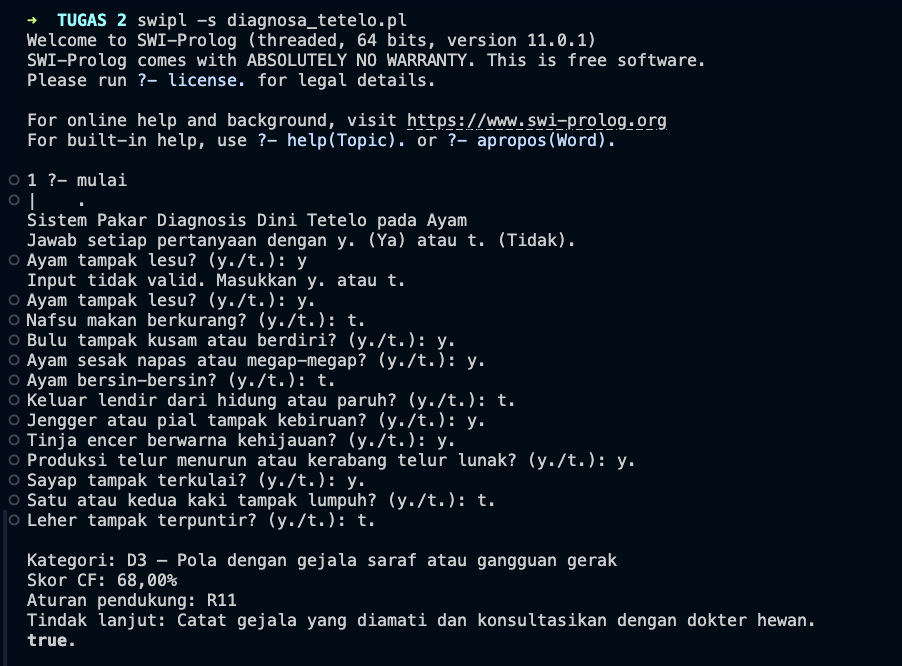
\includegraphics[width=0.92\textwidth]{images/konsol.png}}
\caption{Tangkapan layar eksekusi antarmuka konsol SWI-Prolog (\texttt{diagnosa\_tetelo.pl})}
\label{fig:konsol}
\end{figure}

\section{Antarmuka Web Lokal}
Gambar~\ref{fig:web} memperlihatkan tampilan antarmuka web lokal yang dilayani oleh \texttt{web/server.pl} pada \texttt{http://127.0.0.1:8080/}. Bagian kiri menampilkan lembar pemeriksaan gejala (\texttt{G1}--\texttt{G12}), sedangkan bagian kanan menampilkan hasil skrining kategori \texttt{D3} dengan skor CF \textbf{64,31\%}, tautan rincian perhitungan aturan, dan ringkasan cara kerja metode.

\begin{figure}[H]
\centering
\fbox{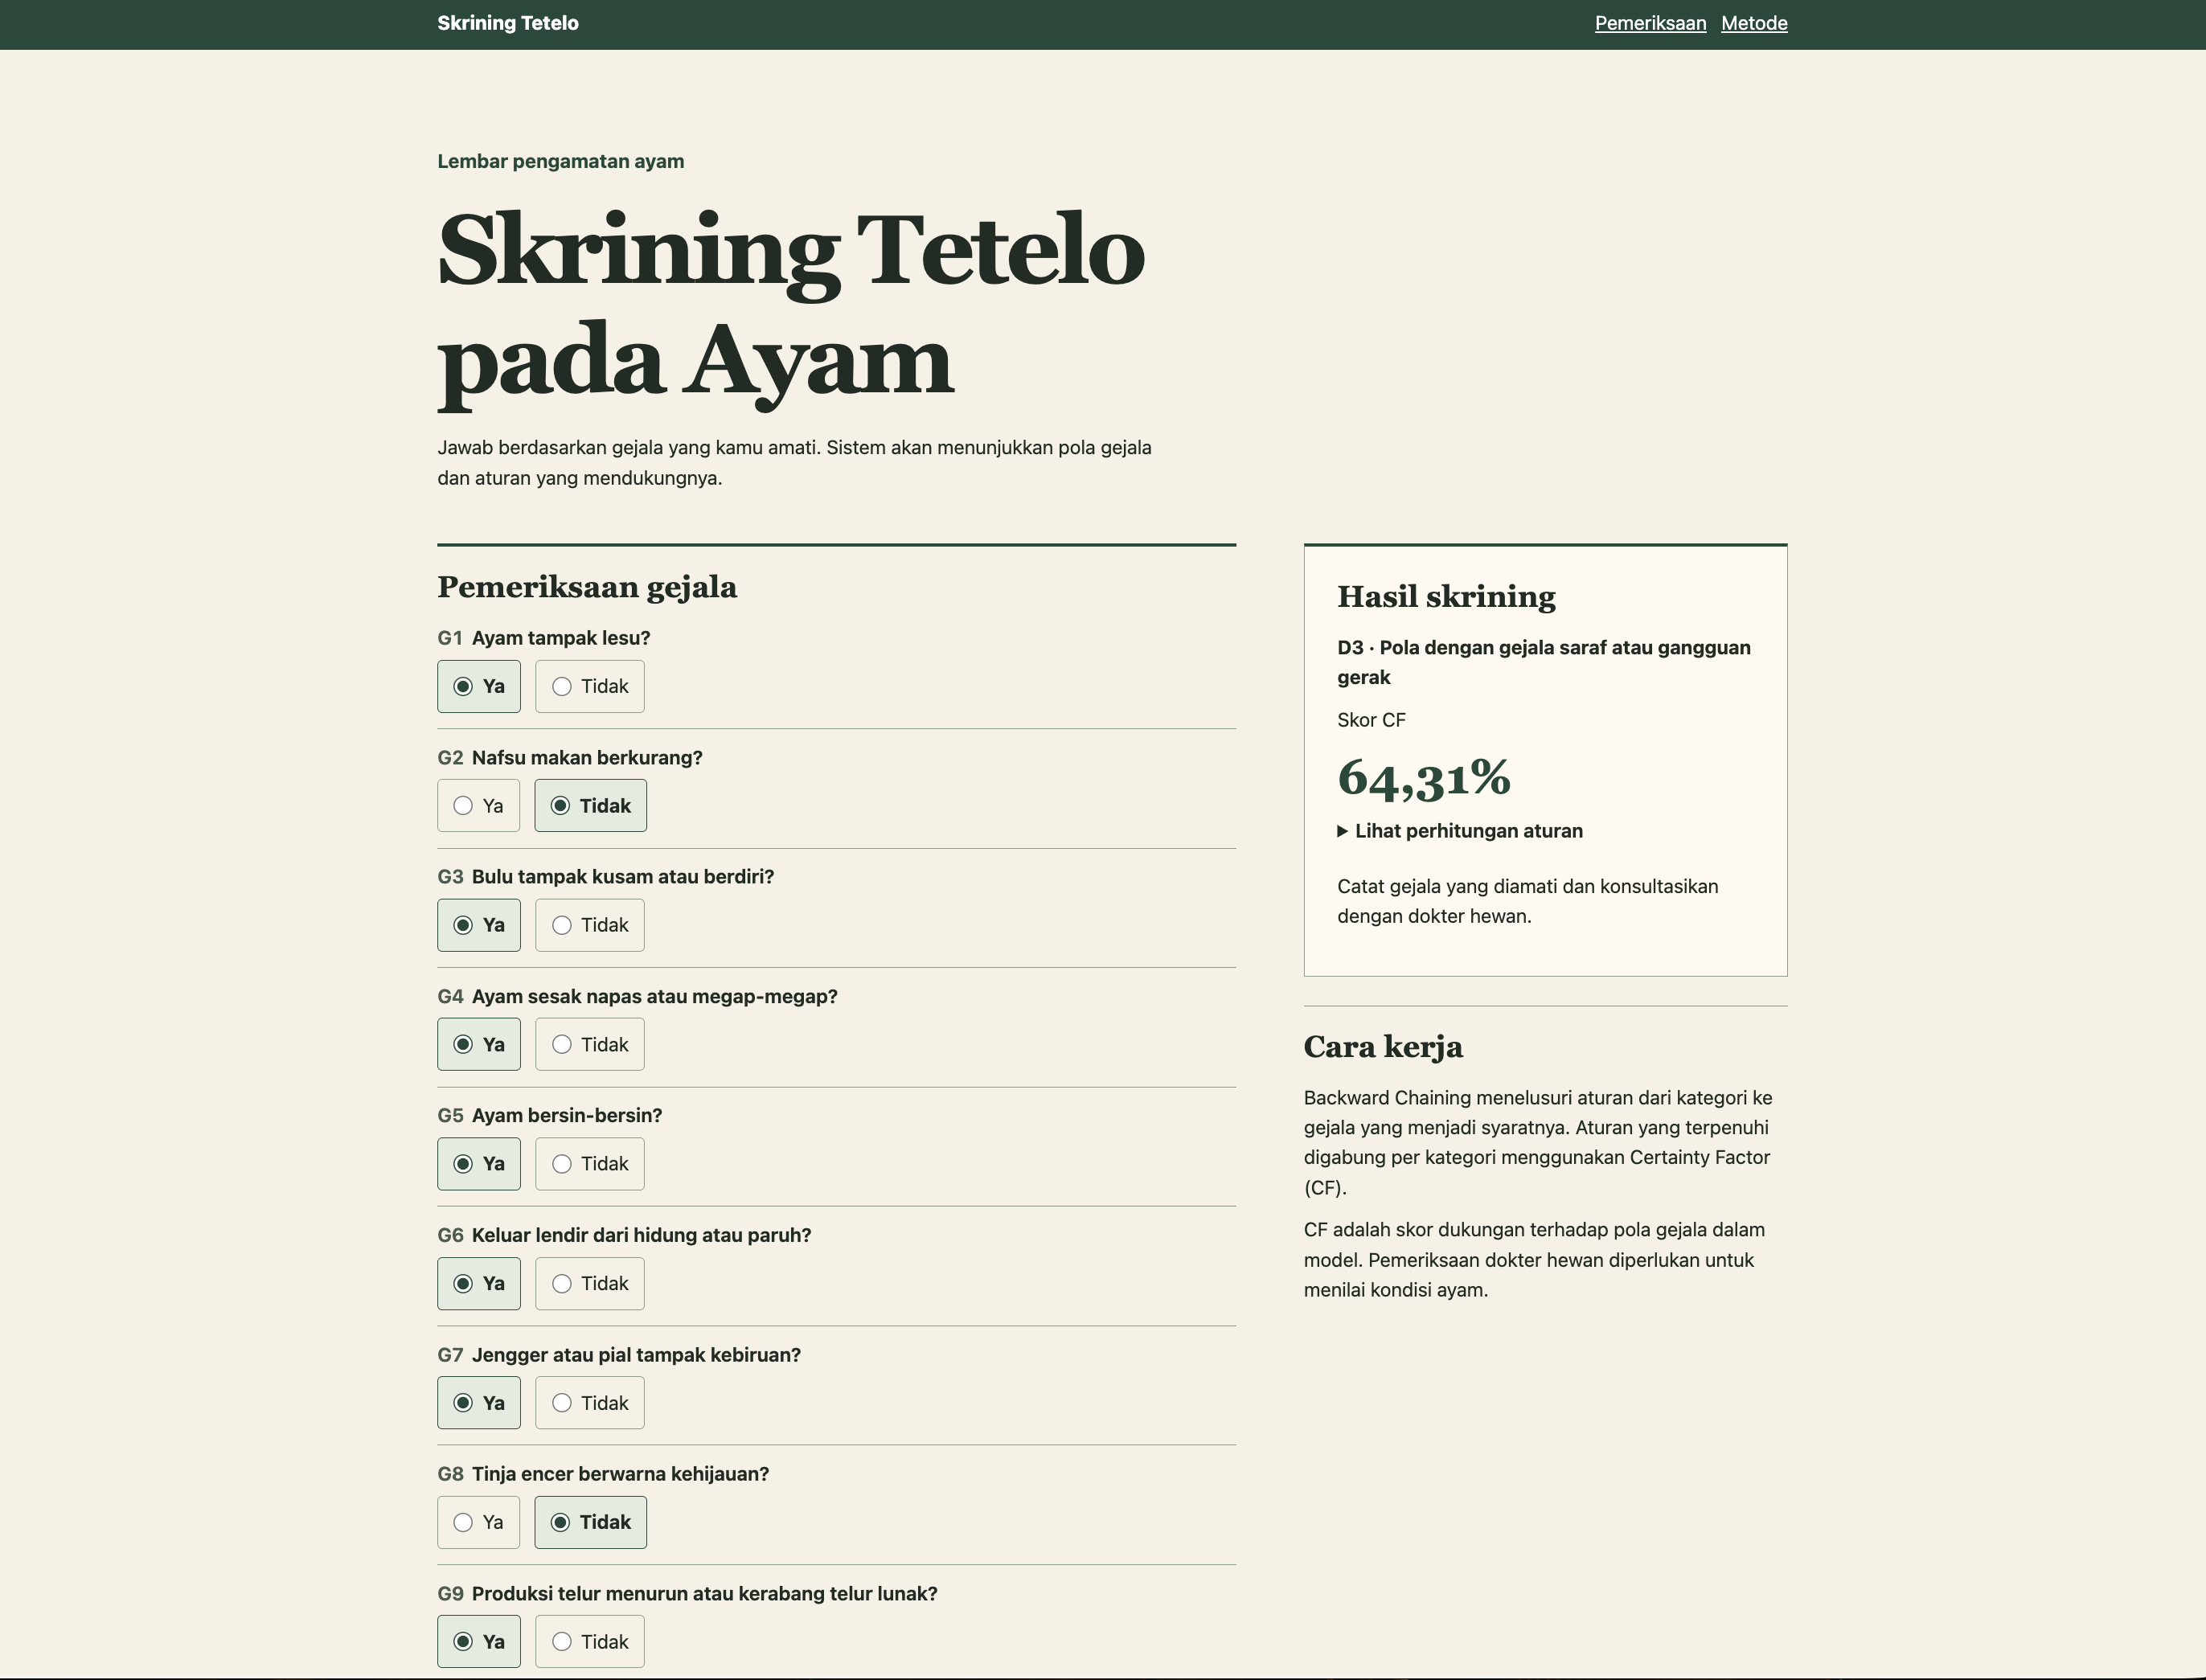
\includegraphics[width=0.95\textwidth]{images/web.png}}
\caption{Tangkapan layar antarmuka web lokal (\texttt{web/server.pl})}
\label{fig:web}
\end{figure}

\end{document}
